\documentclass[tikz,border=10pt]{standalone}
\usepackage{tikz}
\usetikzlibrary{shapes.geometric}

\begin{document}
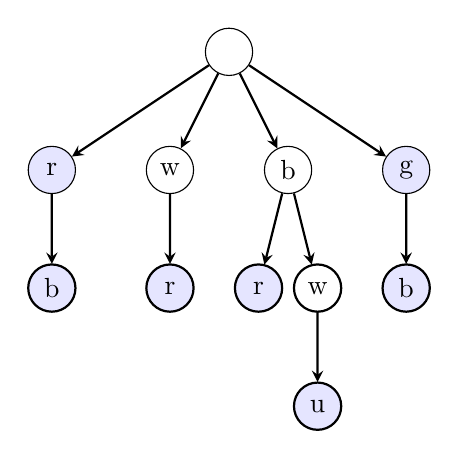
\begin{tikzpicture}[
  edge from parent/.style={
    draw,
    -stealth,
    thick,
  },
  every node/.style={
    draw,
    circle,
    minimum size=6mm,
    inner sep=1pt,
  },
  complete/.style={
    fill=blue!10
  },
  level 1/.style={sibling distance=1.5cm},
  level 2/.style={sibling distance=0.75cm},
]

% Root node
\node[draw] (root) {}
  child {node[complete] (r) {r}
    child {node[complete] (rb) {b}} % Complete word "rb"
  }
  child {node (w) {w}
    child {node[complete] (wr) {r}} % Complete word "wr"
  }
  child {node (b) {b}
    child {node[complete] (br) {r}} % Complete word "br"
    child {node (bw) {w}
      child {node[complete] (bwu) {u}} % Complete word "bwu"
    }
  }
  child {node[complete] (g) {g}
    child {node[complete] (gb) {b}} % Complete word "gb"
  };

\end{tikzpicture}
\end{document}